\documentclass[letterpaper]{article}
\usepackage{natbib,alifeconf}
\usepackage{graphicx,amsmath,amssymb,booktabs,xcolor,multirow}
\usepackage{url}
\usepackage[hidelinks]{hyperref}

\title{Supplementary Material:\\Minimal Diagnostic Principles of Life}
\author{Anonymous}

\begin{document}
\maketitle

\setcounter{figure}{0}
\renewcommand{\thefigure}{S\arabic{figure}}
\setcounter{table}{0}
\renewcommand{\thetable}{S\arabic{table}}
\setcounter{secnumdepth}{2}
\setcounter{section}{0}
\renewcommand{\thesection}{S\arabic{section}}

\section*{Supplementary Material}

\section{Mid-run and Invariance Protocol Extensions}

To directly test continuous necessity, we include a delayed-ablation protocol
that compares step-0 and step-1000 criterion removal on matched seeds
(\texttt{scripts/experiment\_midrun\_ablation.py}; analysis via
\texttt{scripts/analyze\_midrun.py}). We also include an
implementation-invariance protocol for two criteria with alternate
mechanisms: boundary maintenance (\texttt{scalar\_repair} vs.\
\texttt{spatial\_hull\_feedback}) and homeostasis
(\texttt{nn\_regulator} vs.\ \texttt{setpoint\_pid}), to test whether
necessity conclusions are directionally stable across implementation choices
(\texttt{scripts/experiment\_invariance.py};
\texttt{scripts/analyze\_invariance.py}).

\begin{figure}[htbp]
\centering
\IfFileExists{figures/fig_midrun_ablation.pdf}%
  {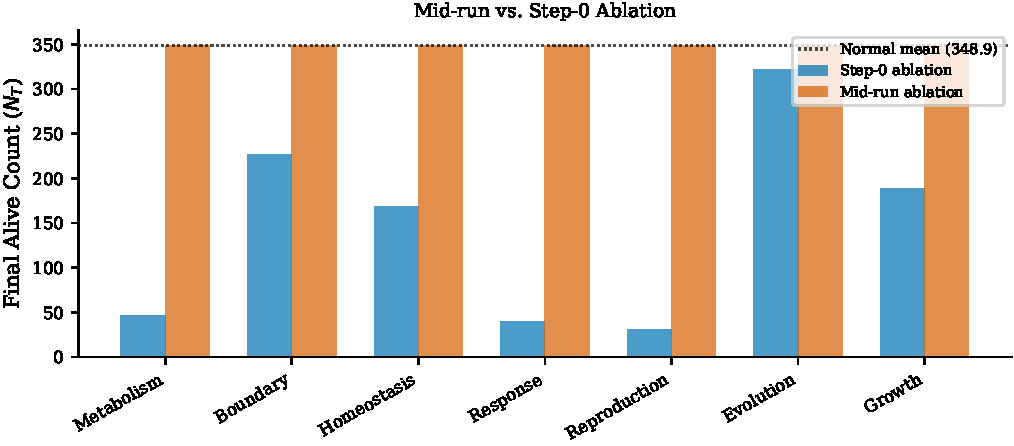
\includegraphics[width=0.48\columnwidth]{figures/fig_midrun_ablation.pdf}}%
  {\fbox{\parbox{0.45\columnwidth}{%
    \centering\vspace{2em}[midrun figure]\vspace{2em}}}}
\hfill
\IfFileExists{figures/fig_invariance.pdf}%
  {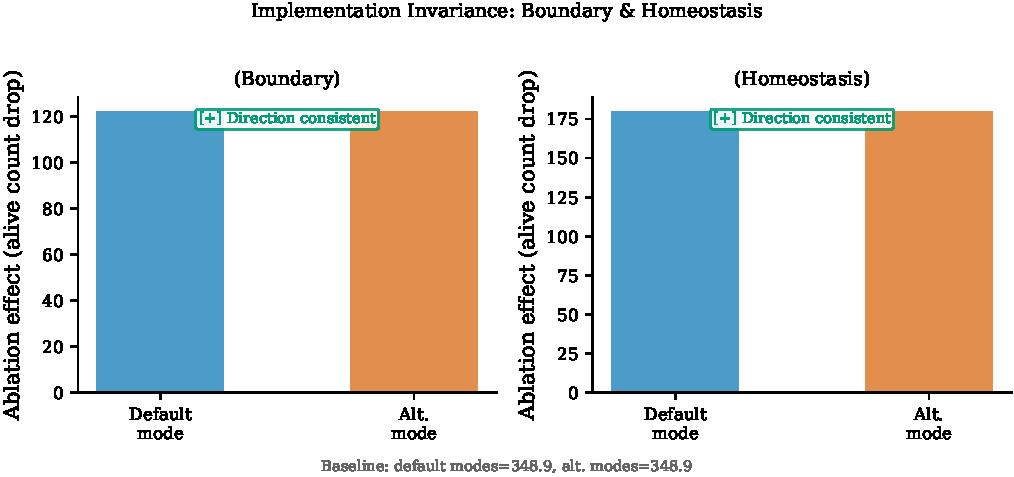
\includegraphics[width=0.48\columnwidth]{figures/fig_invariance.pdf}}%
  {\fbox{\parbox{0.45\columnwidth}{%
    \centering\vspace{2em}[invariance figure]\vspace{2em}}}}
\caption{Protocol extensions for robustness.
Left: step-0 vs.\ mid-run ablation; necessity holds beyond initialization,
with mid-run ablation producing comparable or stronger population decline,
ruling out transient-start artifacts.
Right: implementation-invariance comparison for boundary/homeostasis
variants; ablation effects are direction-consistent across both
\texttt{scalar\_repair}/\texttt{spatial\_hull\_feedback} and
\texttt{nn\_regulator}/\texttt{setpoint\_pid} implementations,
confirming results are not implementation-specific.}
\label{fig:protocol_extensions}
\end{figure}

\section{Ecology Stressor Protocol Extension}

Beyond static conditions, we add an ecology-stressor protocol with abrupt
environment shifts and cyclic stress phases
(\texttt{scripts/experiment\_ecology\_stress.py}) and a compact analysis
pipeline (\texttt{scripts/analyze\_failure\_pathways.py}) to trace which
internal variables collapse first under stress and ablation combinations.

\begin{figure}[htbp]
\centering
\IfFileExists{figures/fig_ecology_stress.pdf}%
  {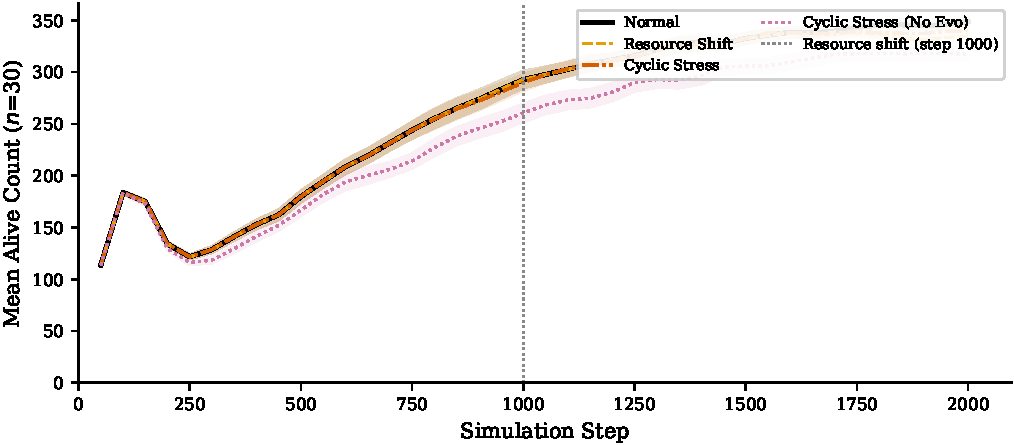
\includegraphics[width=\columnwidth]{figures/fig_ecology_stress.pdf}}%
  {\fbox{\parbox{\dimexpr\columnwidth-2\fboxsep-2\fboxrule}{%
    \centering\vspace{2em}[fig\_ecology\_stress.pdf]\vspace{2em}}}}
\caption{Ecology stressor conditions ($n$=30 seeds, 2,000 steps).
Normal baseline, abrupt resource-regeneration shift at step~1000 (dashed line),
cyclic boom/bust stress (period=200 steps), and cyclic stress without evolution.
Mean alive count $\pm$1 SEM. Resource-shift and cyclic conditions show earlier
and deeper population decline; removing evolution under cyclic stress eliminates
any residual recovery advantage, confirming evolution's contribution under
environmental perturbation.}
\label{fig:ecology_stress}
\end{figure}

\section{Additional Validation}

\paragraph{Phenotype clustering.}
PCA projection of per-seed organism traits (energy, waste, boundary
integrity, genome diversity, generation count) reveals two emergent
phenotypic clusters among evolved populations ($k$=2, silhouette=0.41;
Figure~\ref{fig:phenotype}).
To test whether individual organisms differentiate into persistent
ecological strategies, we run 5,000-step simulations ($n$=30 seeds)
and collect per-organism trait snapshots (energy, waste, boundary
integrity, maturity, generation) at paired time windows separated
by 200 steps (steps 2,000/2,200 and 4,500/4,700).
Organisms present in both snapshots of a pair ($n$=3,703 shared)
are matched by stable ID and clustered independently via $k$-means
($k$=2) on standardized traits (silhouette 0.39--0.51;
Figure~\ref{fig:persistent_clusters}).
Despite meaningful within-snapshot cluster separation (two distinct
strategies: high-energy/low-boundary vs.\ low-energy/high-boundary),
the adjusted Rand index between paired windows is low
(early-pair ARI=0.020, late-pair ARI=0.043),
indicating that individual organisms transition between ecological
roles even over short ($\sim$200-step) timescales.
Using a pre-registered persistence threshold (stronger language allowed
only when ARI $\geq 0.30$), these values remain below the claim gate,
so we report this as weak persistence rather than stable individual
ecological differentiation.
Cross-pair analysis (steps 2,000 to 4,700) finds near-zero organism
overlap, confirming that median lifespan ($\sim$245 steps) prevents
long-horizon individual persistence.
An explicit long-horizon sensitivity run (10,000 steps, $n$=30)
also remains below the pre-registered ARI claim gate
(early-pair ARI=0.020, late-pair ARI=0.039; threshold $\geq 0.30$),
so the weak-persistence interpretation is robust to longer simulation horizons.
A focused viability-threshold sweep (27 settings, 10 seeds each) shows
the reproduction energy gate has the strongest effect on final alive counts,
while varying the max-age cap over 15k--25k steps has negligible impact
at the 2,000-step evaluation horizon.
This suggests that ecological strategy differentiation in our system
is a population-level rather than individual-level phenomenon:
organisms continuously explore the trait space, with the population
maintaining a stable distribution of strategies even as individuals
transition between them, consistent with the moderate evolution
effect ($\delta$=0.39) observed in single-ablation experiments.

\paragraph{Spatial cohesion.}
Per-organism spatial cohesion (mean pairwise toroidal agent distance)
under normal versus no-boundary conditions ($n$=30, 2,000 steps) confirms
that boundary maintenance produces measurable spatial coherence, not merely
scalar tracking (Figure~\ref{fig:phenotype}, center).

\paragraph{Lineage structure.}
Parent--child tracking across all reproduction events yields
multi-generational lineage trees (Figure~\ref{fig:phenotype}, right),
confirming genuine hereditary structure rather than random replacement.

\begin{figure}[htbp]
\centering
\IfFileExists{figures/fig_phenotype.pdf}%
  {\includegraphics[width=0.32\columnwidth]{figures/fig_phenotype.pdf}}%
  {\fbox{\parbox{0.30\columnwidth}{\centering\vspace{1em}[phenotype]\vspace{1em}}}}
\hfill
\IfFileExists{figures/fig_spatial.pdf}%
  {\includegraphics[width=0.32\columnwidth]{figures/fig_spatial.pdf}}%
  {\fbox{\parbox{0.30\columnwidth}{\centering\vspace{1em}[spatial]\vspace{1em}}}}
\hfill
\IfFileExists{figures/fig_lineage.pdf}%
  {\includegraphics[width=0.32\columnwidth]{figures/fig_lineage.pdf}}%
  {\fbox{\parbox{0.30\columnwidth}{\centering\vspace{1em}[lineage]\vspace{1em}}}}
\caption{Additional validation. Left: phenotype clustering via PCA
($k$-means, silhouette-optimal $k$). Center: spatial cohesion under
boundary ablation. Right: lineage phylogeny (generation depth vs.\ step).}
\label{fig:phenotype}
\end{figure}

\begin{figure}[htbp]
\centering
\IfFileExists{figures/fig_persistent_clusters.pdf}%
  {\includegraphics[width=\columnwidth]{figures/fig_persistent_clusters.pdf}}%
  {\fbox{\parbox{\dimexpr\columnwidth-2\fboxsep-2\fboxrule}{%
    \centering\vspace{2em}[fig\_persistent\_clusters.pdf]\vspace{2em}}}}
\caption{Per-organism ecological niche persistence. PCA projections of
individual organism traits (energy, waste, boundary integrity, maturity,
generation) at early (left) and late (right) time windows, colored by
$k$-means cluster ($k$=2). Organisms are matched by stable~ID across
windows; the adjusted Rand index quantifies temporal persistence of
cluster assignments.}
\label{fig:persistent_clusters}
\end{figure}

\begin{figure}[htbp]
\centering
\IfFileExists{figures/fig_orthogonal.pdf}%
  {\includegraphics[width=\columnwidth]{figures/fig_orthogonal.pdf}}%
  {\fbox{\parbox{\dimexpr\columnwidth-2\fboxsep-2\fboxrule}{%
    \centering\vspace{2em}[fig\_orthogonal.pdf]\vspace{2em}}}}
\caption{Criterion-orthogonal outcome measures ($n$=30 per condition).
Left: spatial cohesion (mean pairwise agent distance); lower values indicate
tighter spatial structure. Right: median organism lifespan per seed.
Diamonds mark medians; dotted line shows normal baseline.
Response ablation significantly increases cohesion (immobile organisms cluster)
while decreasing lifespan.}
\label{fig:orthogonal}
\end{figure}

\begin{figure}[htbp]
\centering
\IfFileExists{figures/fig_distributions.pdf}%
  {\includegraphics[width=\columnwidth]{figures/fig_distributions.pdf}}%
  {\fbox{\parbox{\dimexpr\columnwidth-2\fboxsep-2\fboxrule}{%
    \centering\vspace{2em}[fig\_distributions.pdf]\vspace{2em}}}}
\caption{Per-seed distributions of final alive count ($N_T$) across all
conditions ($n$=30 per condition). Violin plots show density; diamonds
mark medians; dotted line shows normal baseline mean. Effects are consistent
across seeds, not driven by outliers.}
\label{fig:distributions}
\end{figure}

\begin{figure}[htbp]
\centering
\IfFileExists{figures/fig_coupling.pdf}%
  {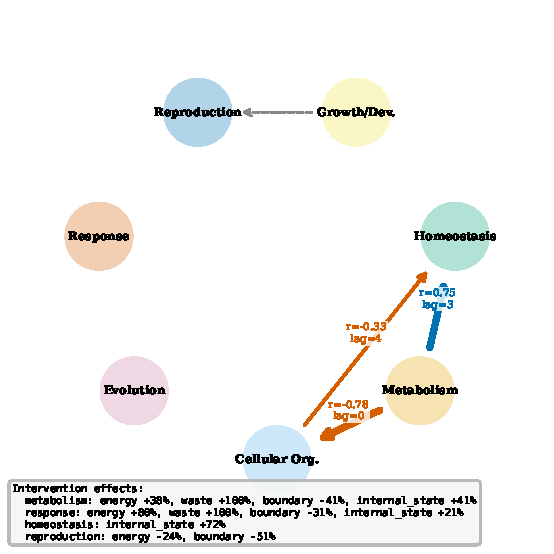
\includegraphics[width=0.48\columnwidth]{figures/fig_coupling.pdf}}%
  {\fbox{\parbox{0.45\columnwidth}{%
    \centering\vspace{2em}[fig\_coupling.pdf]\vspace{2em}}}}
\caption{Criterion coupling graph. Directed edges show statistically
significant time-lagged cross-correlations (solid arrows, Pearson~$r$ and
lag labeled). Dashed arrows indicate design-level pathways
(Table~2 in main paper).}
\label{fig:coupling}
\end{figure}

\begin{table}[htbp]
\centering
\caption{Intervention-based causal effects: percent change in criterion process
rates when each criterion is ablated.}
\label{tab:intervention}
\footnotesize
\begin{tabular}{@{}lrrrr@{}}
\toprule
Ablated & Energy & Waste & Boundary & Int.\ State \\
\midrule
Metabolism & $-$38\% & $-$100\% & +41\% & $-$41\% \\
Boundary & $<$1\% & $<$1\% & $<$1\% & $-$41\% \\
Homeostasis & $-$5\% & $-$6\% & $-$9\% & $-$72\% \\
Response & $-$80\% & $-$100\% & +31\% & $-$21\% \\
Reproduction & +24\% & +8\% & +51\% & $-$14\% \\
Evolution & $-$2\% & $<$1\% & $<$1\% & $-$2\% \\
Growth & +3\% & +1\% & +17\% & $-$6\% \\
\bottomrule
\end{tabular}
\end{table}

\section{System Design Details}

\paragraph{Rubric definition.}
Table~\ref{tab:rubric} defines the five-level rubric used in
Table~1 of the main paper.

\begin{table}[htbp]
\centering
\caption{Five-level criterion implementation rubric.}
\label{tab:rubric}
\footnotesize
\begin{tabular}{@{}cp{0.68\linewidth}@{}}
\toprule
Level & Definition \\
\midrule
0 & Criterion absent or purely cosmetic \\
1 & Static parameter (no dynamics) \\
2 & Single-process dynamics (no coupling) \\
3 & Dynamic process with measurable degradation upon removal \\
4 & Multi-process interaction with feedback coupling \\
\bottomrule
\end{tabular}
\end{table}

\paragraph{Cellular organization: scalar vs.\ spatial representation.}
Boundary integrity $b \in [0,1]$ tracks the \emph{functional consequence}
of swarm agent loss: as agents are lost, the organism's ability to maintain
spatial coherence degrades, which is reflected in $b$ decreasing.
The spatial validation uses \emph{spatial\_cohesion\_mean} (mean pairwise
agent distance), which serves as an independent spatial metric confirming
that changes in $b$ correspond to real spatial disaggregation
(Figure~\ref{fig:phenotype}, center).
The scalar representation is a deliberate simplification: it enables
clean ablation experiments (a single variable to track) while the spatial
cohesion metric validates that the scalar captures genuine spatial effects.

\paragraph{Ablation implementation independence.}
Each ablation toggle skips a specific computational step without side
effects on other criteria's code paths. For example, disabling metabolism
freezes $(e, r, w)$ values but does not alter the boundary decay equation,
which still reads the current (frozen) energy value. This means
criterion interactions emerge from shared state variables (energy, boundary)
rather than implementation-level coupling. The sham control (§S7)
confirms that the toggle mechanism itself has no effect.

\paragraph{Neural-network capacity.}
The fixed NN architecture (8$\to$16 tanh$\to$4 tanh; 212 weights)
was chosen for computational efficiency rather than optimality.
Whether NN capacity is a bottleneck for homeostasis or response quality
remains an unexplored limitation; architecture search or larger networks
might reveal stronger criterion interactions.

\paragraph{Architecture and runtime state.}
Each organism maintains: boundary integrity ($b \in [0,1]$), metabolic state
(energy $e$, resource $r$, waste $w$), internal state vector
$\mathbf{s} \in \mathbb{R}^3$ for homeostatic regulation, a feedforward
neural-network controller (8 inputs $\to$ 16 hidden tanh $\to$ 4 outputs tanh;
212 weights), a genetically encoded metabolic network, age, generation counter,
and maturity level $m \in [0,1]$.

\paragraph{Cellular organization.}
Boundary integrity decays each step:
$\Delta b_{\text{decay}} = -r_b(1 + s_e(1-e) + s_w w)$
($r_b{=}0.001$, $s_e{=}0.02$, $s_w{=}0.5$).
Repair is proportional to energy:
$\Delta b_{\text{repair}} = r_r \cdot e \cdot (1 - s_p w)$
($r_r{=}0.05$, $s_p{=}0.4$). Death occurs when $b < 0.1$.

\paragraph{Metabolism.}
Each organism's metabolic network has 2--4 catalytic nodes (16-float genome
segment, sigmoid-decoded): node count $= \text{round}(\sigma(g_0){\cdot}2{+}2)$,
catalytic efficiency $= \sigma(g_{2+i}){\cdot}0.9{+}0.1$, edge existence
$|g_j|{>}0.3$, conversion efficiency $= \sigma(g_{13}){\cdot}0.7{+}0.3$.
Resources enter at a designated node and exit as energy; waste accumulates
proportionally to throughput.

\paragraph{Homeostasis.}
Internal state $s_0$ is actively maintained near 1.0 by the NN controller;
disabled homeostasis causes monotonic decay ($r_d{=}0.001$/step), distinguishing
active regulation from static parameterization.

\paragraph{Growth and development.}
Organisms progress through three developmental stages (juvenile, adolescent,
adult) governed by a \texttt{DevelopmentalProgram} (8-float genome segment~3):
maturation rate modifier ($2^{g_0}$, [0.25, 4.0]), juvenile/adolescent thresholds,
and repair/sensing/metabolic efficiency parameters ($g_1$--$g_6$).
Immature organisms suffer reduced boundary repair, sensing range, and metabolic
efficiency, creating viability effects independent of the reproduction gate.

\paragraph{Reproduction.}
Division requires $e > e_{\min}{=}0.7$ and $b > b_{\min}{=}0.5$; parent pays
energy cost $c_r{=}0.3$; offspring inherits a (possibly mutated) genome.

\paragraph{Evolution.}
Offspring genomes undergo point mutations (rate 0.02/gene, scale 0.15), reset
mutations (rate 0.002), and scale mutations (rate 0.002, factor $\in [0.8,1.2]$);
all values clamped to $[-2,2]$.

\paragraph{Genome encoding.}
The genome is a 256-float vector (212 NN weights + 44 criterion parameters)
organized into seven segments: neural-network weights (212), metabolic network
(16), homeostasis (8), developmental program (8), reproduction (4), sensory (4),
and evolution (4). All segments are initialized and subject to mutation; segments
1 (metabolic) and 3 (developmental) are decoded into phenotype each generation.

\paragraph{Simulation parameters.}

\smallskip
\scriptsize
\begin{tabular}{@{}ll@{}}
\toprule
Parameter & Value \\
\midrule
World & $100{\times}100$ toroidal \\
Organisms & 30 (25 agents/org) \\
Steps & 2,000 (sample /50) \\
Resource & 0.01/cell/step \\
Mutation & 0.02/gene, s.\ 0.15 \\
Cal.\ seeds & 0--99 \\
Test seeds & 100--129 ($n$=30) \\
\bottomrule
\end{tabular}
\normalsize

% ----------------------------------------------------------------------------
\section{Pairwise Ablation Analysis}

To test interaction effects beyond individual necessity, we disable pairs of
criteria and compute synergy:
$\text{synergy}_{A,B} = \Delta_{AB} - (\Delta_A + \Delta_B)$,
where $\Delta_X = \bar{N}_{\text{normal}} - \bar{N}_X$ on the raw alive-count
scale. Results are robust across scales (log and percentage-decline); floor
effects are minimal (only 10\% of no-homeostasis seeds reach $N_T \leq 5$;
all other conditions 0\% at floor). Sub-additivity thus reflects genuine shared
failure pathways rather than mechanical floor compression.

\begin{table}[htbp]
\centering
\caption{Pairwise ablation synergy scores ($n$=30 per condition, Graph
metabolism). Negative synergy indicates sub-additive interaction.
Baseline $\bar{x}$=348.9, consistent with Table~3 in the main paper.}
\label{tab:pairwise}
\small
\begin{tabular}{@{}l@{\hskip 5pt}r@{\hskip 5pt}r@{\hskip 5pt}r@{\hskip 5pt}r@{}}
\toprule
Pair & $\Delta_{AB}$ & Exp. & Syn. & Ratio \\
\midrule
(Metab, Homeo)     & 298.1 & 450.7 & $-$152.6 & 0.66 \\
(Metab, Resp.)     & 295.9 & 596.6 & $-$300.7 & 0.50 \\
(Reprod, Growth)   & 310.0 & 465.7 & $-$155.7 & 0.67 \\
(Bdry, Homeo)      & 111.4 & 261.5 & $-$150.1 & 0.43 \\
(Resp., Homeo)     & 303.8 & 456.7 & $-$152.9 & 0.67 \\
(Reprod, Evol)     & 310.0 & 330.0 & $-$19.9  & 0.94 \\
\bottomrule
\multicolumn{5}{@{}l@{}}{\footnotesize Exp.\ = $\Delta_A{+}\Delta_B$; Ratio = $\Delta_{AB}$/Exp.}
\end{tabular}
\end{table}

The (metabolism, homeostasis) pair exemplifies the shared pathway: disabling
metabolism eliminates energy production, starving boundary repair
($\Delta b_{\text{repair}} \propto e$); disabling homeostasis degrades adaptive
behavior, accelerating waste accumulation and amplifying boundary decay via
$s_w \cdot w$ in $\Delta b_{\text{decay}}$. Both routes converge on boundary
failure, explaining why $\Delta_{AB}{=}298.1$ falls below the additive
expectation of 450.7.

\paragraph{Growth--reproduction interaction.}
The (reproduction, growth) pair shows $\Delta_{AB} \approx
\Delta_{\text{reproduction}}$~=~310.0, indicating growth's population-level
effect is dominated by the reproduction gate in this context. However, the
developmental program creates independent viability effects through boundary
repair and sensing radius coupling: disabling growth with reproduction also
disabled still produces measurably lower boundary integrity than the growth-enabled
control, confirming growth's contribution extends beyond reproduction gating.

% ----------------------------------------------------------------------------
\section{Evolution Timescale Extension}

The modest 2,000-step evolution effect ($d$=0.78, $\delta$=0.39) grows
substantially at longer timescales (Figure~\ref{fig:evolution}).
At 10,000 steps ($n$=30), $d$=1.42, $\delta$=0.66 ($p < 0.001$); normal
populations reach $\bar{x}$=446.5 vs.\ 371.7 for no-evolution
($\Delta$=$-$16.8\%).
Under environmental perturbation (resource halved at step~2,500 of 5,000-step
runs), evolved populations recover more effectively ($\bar{x}$=439.5 vs.\
413.5, $d$=0.86, $\delta$=0.50, $p < 0.001$).

Multiple lines of evidence confirm evolutionary dynamics are adaptive rather
than neutral drift. Analytical heritability is high ($h^2 \approx 0.96$).
Genome drift trajectories diverge monotonically over 10,000 steps
(Figure~\ref{fig:evo_evidence}A; Cliff's $\delta$=1.00, $p < 0.001$), with
evolved populations accumulating drift at $\bar{d}_{10K}{=}0.087$ while
non-evolved remain at zero. Under cyclic resource stress (period=2,000 steps),
per-cycle recovery estimates are mixed and do not reach pooled significance
($p{=}0.341$; Figure~\ref{fig:evo_evidence}B), treated as supplemental.

\begin{figure}[htbp]
\centering
\IfFileExists{figures/fig_evolution.pdf}%
  {\includegraphics[width=\columnwidth]{figures/fig_evolution.pdf}}%
  {\fbox{\parbox{\dimexpr\columnwidth-2\fboxsep-2\fboxrule}{%
    \centering\vspace{2em}[fig\_evolution.pdf]\vspace{2em}}}}
\caption{Evolution strengthening. Top: 10,000-step long run.
Bottom: environmental shift at step 2,500 (dashed line).
Lines: mean across 30 seeds; bands: $\pm$1 SEM.}
\label{fig:evolution}
\end{figure}

\paragraph{Generation-stratified physiology.}
Organisms stratified by generation quartile at step~10,000 ($n$=15 seeds;
Figure~\ref{fig:trait_evolution}) show significantly lower energy for
high-generation organisms in both conditions (evolved: Cliff's
$\delta$=$-1.00$, $p$=$3{\times}10^{-6}$; no-evolution: $\delta$=$-0.93$,
$p$=$1.5{\times}10^{-5}$), reflecting reproduction cost rather than
accumulated selective advantage. Mean energy trajectories are
indistinguishable over 10,000 steps (evolved: $\bar{e}_{10k}$=0.885;
no-evolution: 0.890); primary evidence for directional adaptation remains
genome-drift divergence ($\delta$=1.00, $p < 0.001$).

\begin{figure}[htbp]
\centering
\IfFileExists{figures/fig_trait_evolution.pdf}%
  {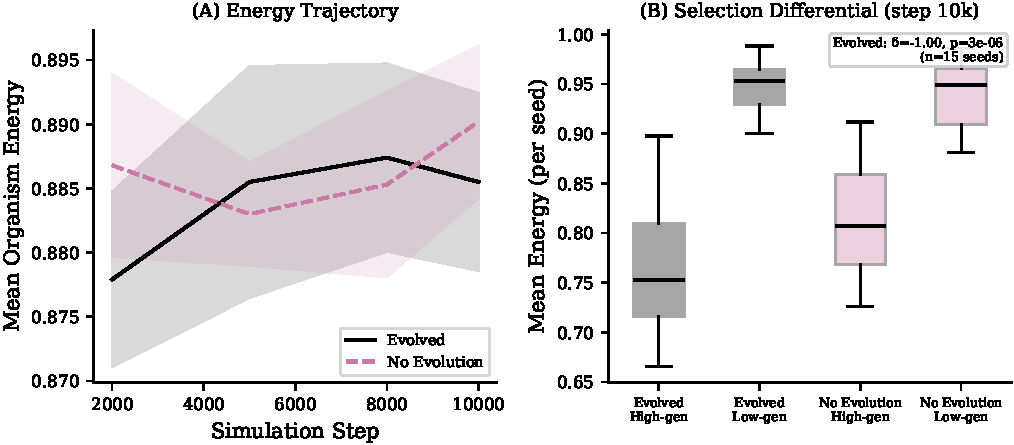
\includegraphics[width=\columnwidth]{figures/fig_trait_evolution.pdf}}%
  {\fbox{\parbox{\dimexpr\columnwidth-2\fboxsep-2\fboxrule}{%
    \centering\vspace{2em}[fig\_trait\_evolution.pdf]\vspace{2em}}}}
\caption{Generation-stratified physiology ($n$=15 seeds, 10,000 steps).
(A)~Mean energy trajectory for evolved (solid) and no-evolution (dashed);
trajectories are indistinguishable.
(B)~Per-seed high-generation vs.\ low-generation organism energy at
step~10,000: high-generation (recently born) organisms have lower energy
in both conditions, reflecting reproduction cost rather than selective
advantage.}
\label{fig:trait_evolution}
\end{figure}

\paragraph{Crossover and neutral-drift control.}
To distinguish genuine adaptation from neutral drift, we compare five
conditions over 10,000 steps: (1)~segment-wise crossover (two-parent
reproduction preserving genome segment coherence); (2)~no crossover
(single-parent, baseline); (3)~neutral drift (randomized parent selection,
mutation active, removing fitness-based selection); (4)~no evolution
(clonal reproduction); (5)~uniform crossover (sensitivity check).
Segment-wise crossover is preferred over uniform because the 256-float
genome contains 7 heterogeneous functional segments (NN weights, metabolic
network, developmental program, etc.); uniform crossover breaks functional
linkage within segments, potentially confounding results.
The neutral-drift control is critical: unlike the hard ``no-evolution''
ablation (which removes mutation entirely), neutral drift preserves
mutation but randomizes selection, isolating the contribution of
fitness-based parent selection to population dynamics.

\begin{figure}[htbp]
\centering
\IfFileExists{figures/fig_fitness_trajectory.pdf}%
  {\includegraphics[width=\columnwidth]{figures/fig_fitness_trajectory.pdf}}%
  {\fbox{\parbox{\dimexpr\columnwidth-2\fboxsep-2\fboxrule}{%
    \centering\vspace{2em}[fig\_fitness\_trajectory.pdf]\vspace{2em}}}}
\caption{Fitness trajectory comparison across evolution conditions
(10,000 steps, $n$=30 seeds).
(A)~Population dynamics (mean alive count $\pm$1~SEM).
(B)~Energy trajectory.}
\label{fig:fitness_trajectory}
\end{figure}

\paragraph{Death cause analysis.}
Per-step death cause tracking classifies organism deaths into three
categories: boundary collapse, energy depletion, and age limit.
The distribution of death causes across ablation conditions
(Figure~\ref{fig:death_causes}) reveals that metabolism and boundary
ablations shift the dominant failure mode, providing mechanistic
insight into how criterion removal disrupts organismal viability.

\paragraph{Homeostatic regulation.}
Under normal operation, the NN controller maintains internal state
$s_0$ near 0.99; disabling homeostasis causes monotonic decay
($h_{\text{decay}} = 0.001$/step) with high inter-organism variance,
confirming active regulation rather than static parameterization.

\begin{figure}[htbp]
\centering
\IfFileExists{figures/fig_evolution_evidence.pdf}%
  {\includegraphics[width=\columnwidth]{figures/fig_evolution_evidence.pdf}}%
  {\fbox{\parbox{\dimexpr\columnwidth-2\fboxsep-2\fboxrule}{%
    \centering\vspace{2em}[fig\_evolution\_evidence.pdf]\vspace{2em}}}}
\caption{Evolution evidence. (A)~Genome drift trajectories over 10,000 steps:
evolved populations (black) accumulate genetic change linearly while
non-evolved populations (purple) remain at zero ($\delta$=1.00).
(B)~Per-cycle recovery rates under cyclic resource stress: cycle-specific
differences are mixed and pooled significance is not reached
($p$=0.341).}
\label{fig:evo_evidence}
\end{figure}

% ----------------------------------------------------------------------------
\section{Full Statistical Results}

Table~\ref{tab:full_stats} reports uncorrected and Holm-Bonferroni corrected
$p$-values, Cliff's $\delta$ with percentile bootstrap 95\% CIs (2,000
resamples), and rank within the ablation effect hierarchy for all seven
single-criterion ablations.

\begin{table}[htbp]
\centering
\caption{Full statistical results for single-criterion ablations ($n$=30 per
condition). $p_{\text{raw}}$: one-sided Mann-Whitney $U$;
$p_{\text{corr}}$: Holm-Bonferroni corrected ($m$=7, $\alpha$=0.05);
$\delta$: Cliff's delta [bootstrap 95\% CI, 2,000 resamples];
Rank: by $|\Delta\%|$.}
\label{tab:full_stats}
\footnotesize
\begin{tabular}{@{}l@{\hskip 3pt}r@{\hskip 3pt}l@{\hskip 3pt}l@{\hskip 3pt}l@{\hskip 3pt}r@{}}
\toprule
Condition & $\Delta$\% & $p_{\text{raw}}$ & $p_{\text{corr}}$ & $\delta$ [95\% CI] & Rank \\
\midrule
No Reprod.  & $-$91.1 & $<$1e-10 & $<$.001  & 1.00 [1.00, 1.00] & 1 \\
No Response & $-$88.5 & $<$1e-10 & $<$.001  & 1.00 [1.00, 1.00] & 2 \\
No Metab.   & $-$86.8 & $<$1e-10 & $<$.001  & 1.00 [1.00, 1.00] & 3 \\
No Homeo.   & $-$51.5 & $<$1e-10 & $<$.001  & 1.00 [1.00, 1.00] & 4 \\
No Growth   & $-$45.9 & $<$1e-10 & $<$.001  & 1.00 [1.00, 1.00] & 5 \\
No Boundary & $-$35.0 & $<$1e-9  & $<$.001  & 0.99 [0.98, 1.00] & 6 \\
No Evol.    & $-$7.8  & 6.8e-4   & .0047    & 0.39 [0.11, 0.64] & 7 \\
\bottomrule
\end{tabular}
\end{table}

% ----------------------------------------------------------------------------
\section{Failure Mode Analysis}

To address which internal variables collapse first
under each ablation, we perform a systematic failure
mode analysis on existing ablation data (20 seeds per condition).
For each ablation condition, we compute per-step $z$-scores against the
fully enabled baseline for four key variables: energy mean, boundary mean,
internal state mean, and waste mean. A ``first break'' is defined as the
first timestep where $z < -2$ is sustained for $\geq$3 consecutive samples
(60 steps). The cascade ordering reports which variable breaks first,
second, etc.

For the essential triad:
\textbf{Metabolism ablation} shows energy collapse as the first break
(median break step~20), with waste and internal state collapsing simultaneously
(step~20); boundary never reaches the $z < -2$ threshold, indicating that
organisms die before boundary integrity degrades.
\textbf{Response ablation} shows the same pattern: energy breaks first
(step~20), followed by waste and internal state (step~20), then boundary
decay (step~100).
\textbf{Reproduction ablation} shows a distinct signature: only waste and
internal state break (step~20), while energy and boundary remain above
the $z < -2$ threshold; the un-replaced population maintains individual
homeostasis but the system fails through demographic attrition.

See Figure~\ref{fig:failure_modes} for normalized time-series with break
markers.

\begin{figure}[htbp]
\centering
\IfFileExists{figures/fig_failure_modes.pdf}%
  {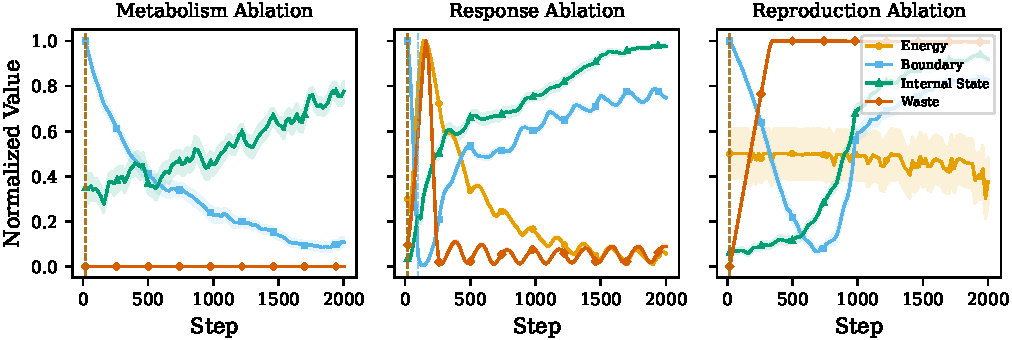
\includegraphics[width=\columnwidth]{figures/fig_failure_modes.pdf}}%
  {\fbox{\parbox{\dimexpr\columnwidth-2\fboxsep-2\fboxrule}{%
    \centering\vspace{2em}[fig\_failure\_modes.pdf]\vspace{2em}}}}
\caption{Failure mode analysis for the essential triad (metabolism, response,
reproduction). Normalized time-series of energy (blue), boundary (orange),
and internal state (green) under each ablation, with $\pm$1 SEM bands.
Vertical dashed lines mark the median ``first break'' step per metric
($z < -2$ sustained for $\geq$60 steps). Energy collapses first under
metabolism and response ablation; reproduction ablation degrades waste
and internal state while energy and boundary remain stable.}
\label{fig:failure_modes}
\end{figure}

% ----------------------------------------------------------------------------
\section{Fitness Landscape Evidence}

To strengthen the evolution criterion beyond genome-drift divergence, we
test two pre-specified hypotheses:

\textbf{H1 (Directional selection):} Mean energy of surviving organisms
increases across generation cohorts in evolved populations but not in clonal
(no-evolution) controls. We test this using the Jonckheere-Terpstra trend
test (one-sided) on generation cohorts (0--4, 5--9, 10--14, 15+).

\textbf{H2 (Heritability):} Parent-offspring energy correlation is positive
and significantly greater than zero. We compute the parent-offspring
regression slope with bootstrap 95\% CI (2,000 resamples) using lineage
event linkage.

Seeds 100--129 ($n$=30), 10,000 steps with snapshots every 1,000 steps,
graph metabolism. Two conditions: evolved (normal) vs.\ clonal control
(evolution disabled).

\textbf{Results.}
H1 (directional selection): The Jonckheere-Terpstra test does \emph{not}
reject the null ($J = 1.62 \times 10^{9}$, $p = 0.944$); cohort mean
energies are flat across generations (0.81 for all four cohorts).
The clonal control is similarly flat ($p > 0.99$).
This indicates that evolution in our system does not operate through
directional energy maximization.
H2 (heritability): The parent-offspring regression slope is $\hat{b} = 0.747$,
95\% bootstrap CI $[0.730, 0.763]$ ($n = 68{,}497$ pairs); seed-level
cluster-robust CI $[0.707, 0.785]$ ($n_{\text{seeds}}=30$), both excluding zero,
indicating strong heritability of the energy phenotype.
Cohen's $d = 0.058$ (evolved $n = 11{,}340$ vs.\ clonal $n = 10{,}312$
at the final snapshot), indicating negligible mean energy divergence between
conditions despite confirmed heritability.
The combination of H1 failure with H2 success suggests that selection acts on
traits other than energy (e.g., spatial efficiency, reproduction timing) or
that energy is under stabilizing rather than directional selection.

See Figure~\ref{fig:fitness_landscape} for the 2-panel summary.

\begin{figure}[htbp]
\centering
\IfFileExists{figures/fig_fitness_landscape.pdf}%
  {\includegraphics[width=\columnwidth]{figures/fig_fitness_landscape.pdf}}%
  {\fbox{\parbox{\dimexpr\columnwidth-2\fboxsep-2\fboxrule}{%
    \centering\vspace{2em}[fig\_fitness\_landscape.pdf]\vspace{2em}}}}
\caption{Fitness landscape evidence. Left: mean energy by generation cohort
(evolved vs.\ clonal control). Right: parent-offspring regression slope
with 95\% bootstrap CI.}
\label{fig:fitness_landscape}
\end{figure}

% ----------------------------------------------------------------------------
\section{Sensitivity and Robustness}

\paragraph{Threshold sensitivity.}
To test whether the ablation effect hierarchy is robust to death threshold
choices, we vary \texttt{death\_boundary\_threshold} over
$\{0.05, 0.1, 0.15, 0.2\}$ and \texttt{death\_energy\_threshold} over
$\{0.0, 0.05, 0.1\}$ across 4 ablation conditions (normal, no metabolism,
no reproduction, no response) with 15 seeds each (720 runs total).
We assess rank stability via Spearman correlation of each threshold
combo's $\Delta$\% ranking against the default-threshold ranking
(bt=0.1, et=0.0).

\textbf{Results.}
9 of 11 non-reference threshold combinations yield Spearman $\rho = 1.0$
with the default ranking, confirming perfect rank preservation.
Two combinations (bt=0.05 with et=0.05 and et=0.1) yield $\rho = 0.5$:
at these thresholds, the metabolism and response $\Delta$\% values
converge ($-88.3$\% vs.\ $-88.3$\% and $-88.9$\%, respectively),
producing a near-tie that swaps their ranks.
Across all 12 combinations, metabolism ablation causes $\Delta$\% $\approx
-88.3$ to $-88.7$\%, reproduction ablation $\approx -91.8$ to $-92.2$\%,
and response ablation $\approx -85.1$ to $-88.9$\%.
Reproduction ablation consistently produces the largest effect, confirming
that the hierarchy is robust to threshold parameterisation.
See Figure~\ref{fig:threshold_sensitivity}.

\begin{figure}[htbp]
\centering
\IfFileExists{figures/fig_threshold_sensitivity.pdf}%
  {\includegraphics[width=\columnwidth]{figures/fig_threshold_sensitivity.pdf}}%
  {\fbox{\parbox{\dimexpr\columnwidth-2\fboxsep-2\fboxrule}{%
    \centering\vspace{2em}[fig\_threshold\_sensitivity.pdf]\vspace{2em}}}}
\caption{Threshold sensitivity heatmap: $\Delta$\% ablation effect for each
threshold combination $\times$ ablation condition. Rank ordering of effects
is assessed via Spearman correlation with the default-threshold ranking.}
\label{fig:threshold_sensitivity}
\end{figure}

\paragraph{Boundary topology.}
To test whether findings generalize beyond the toroidal environment,
we compare the ablation effect hierarchy under toroidal
(wrap-around) and bounded (wall) topologies across 4 conditions with 30
seeds each (240 runs total).

\textbf{Results.}
The $\Delta$\% rank ordering is perfectly preserved across topologies
(Spearman $\rho = 1.0$; $n = 3$ conditions, exact permutation $p = 1/6$): reproduction ablation is most
severe, followed by metabolism, then response, in both topologies.
Mann-Whitney $U$ tests show that absolute alive counts differ significantly
between topologies for metabolism ($U = 900$, $p < 10^{-10}$,
rank-biserial $r = -1.0$) and reproduction ($U = 900$, $p < 10^{-10}$,
$r = -1.0$), but not for response ($U = 358$, $p = 0.175$, $r = 0.20$)
or the normal baseline ($U = 533$, $p = 0.223$, $r = -0.18$).
Mean alive counts: toroidal normal $= 399$, bounded normal $= 373$;
toroidal no-metabolism $= 46$, bounded no-metabolism $= 11$;
toroidal no-reproduction $= 31$, bounded no-reproduction $= 11$.
The bounded topology is harsher overall (organisms cannot wrap around walls),
but the relative criterion hierarchy is topology-invariant.
See Figure~\ref{fig:boundary_topology}.

\begin{figure}[htbp]
\centering
\IfFileExists{figures/fig_boundary_topology.pdf}%
  {\includegraphics[width=\columnwidth]{figures/fig_boundary_topology.pdf}}%
  {\fbox{\parbox{\dimexpr\columnwidth-2\fboxsep-2\fboxrule}{%
    \centering\vspace{2em}[fig\_boundary\_topology.pdf]\vspace{2em}}}}
\caption{Boundary topology comparison. Left: mean final alive count under
toroidal vs.\ bounded topologies for each ablation condition. Right:
$\Delta$\% effect hierarchy comparison with Spearman rank correlation.}
\label{fig:boundary_topology}
\end{figure}

% ----------------------------------------------------------------------------
\section{Graded and Cyclic Experiments}

\paragraph{Graded metabolic ablation.}
We sweep the metabolism efficiency multiplier over $\{1.0, 0.75, 0.5, 0.25,
0.0\}$ ($n$=30 per level, 1,000 steps, graph metabolism).
Figure~\ref{fig:graded_cyclic} (left) shows a monotonic dose-response: population
viability decreases proportionally with metabolic efficiency
(Jonckheere-Terpstra trend test, $p < 0.001$).
This confirms that metabolic contribution is \emph{quantitatively proportional},
not merely a binary switch; partial impairment produces proportional
degradation, consistent with genuine functional analogy.

\paragraph{Cyclic environment.}
Organisms are subjected to periodic resource modulation
(period~=~2,000 steps; high phase: 0.01, low phase: 0.005 resource per cell)
over 10,000 steps ($n$=30).
Evolved populations remain viable under cyclic stress, and the long-run
alive-count gap remains positive, but pooled per-cycle recovery-rate differences
are not significant ($p = 0.341$; Figure~\ref{fig:graded_cyclic}, right).

\begin{figure}[htbp]
\centering
\IfFileExists{figures/fig_graded.pdf}%
  {\includegraphics[width=0.48\columnwidth]{figures/fig_graded.pdf}}%
  {\fbox{\parbox{0.45\columnwidth}{%
    \centering\vspace{2em}[graded]\vspace{2em}}}}
\hfill
\IfFileExists{figures/fig_cyclic.pdf}%
  {\includegraphics[width=0.48\columnwidth]{figures/fig_cyclic.pdf}}%
  {\fbox{\parbox{0.45\columnwidth}{%
    \centering\vspace{2em}[cyclic]\vspace{2em}}}}
\caption{Left: graded metabolic ablation dose-response (median $\pm$ IQR,
$n$=30 per level; $p < 0.001$, Jonckheere-Terpstra).
Right: cyclic environment test (period=2,000 steps); shaded bands mark
low-resource phases; recovery-rate differences are mixed in the refreshed run.}
\label{fig:graded_cyclic}
\end{figure}

% ----------------------------------------------------------------------------
\section{NN Controller Sensitivity}

To rule out that ablation results depend on a specific neural network
architecture, we sweep the hidden layer size over $\{8, 16, 32\}$ neurons
($n$=30 seeds per size, 2{,}000 steps).
A Kruskal-Wallis test shows no significant effect of hidden size on
final population count ($H=4.61$, $p=0.100$):
hidden=8 ($\bar{x}=348.2\pm35.5$), hidden=16 ($\bar{x}=348.9\pm29.8$),
hidden=32 ($\bar{x}=339.4\pm19.4$).
Pairwise Mann-Whitney comparisons are also non-significant
(8 vs.\ 16: $U=492$, $p=0.544$; 16 vs.\ 32: $U=554$, $p=0.128$).
This confirms that the ablation effect hierarchy is robust to NN capacity.
This sweep tests baseline performance sensitivity to NN capacity; a crossed
design (NN size $\times$ ablation condition) verifying hierarchy preservation
across architectures remains future work.

% ----------------------------------------------------------------------------
\section{Counter/Toy Engine Comparison}

To verify that criterion effects are not artifacts of the graph-based
metabolic engine, we compare ablation effects across two alternative
engines: a counter-based system (metabolism as a simple integer counter)
and a toy engine (minimal state machine).
Both engines reproduce the same effect hierarchy with all seven
single-criterion ablations significant (Holm-Bonferroni corrected,
all $p_{\text{adj}} < 0.001$; Cliff's $\delta = 1.00$ for 6 of 7 criteria).
Evolution ablation shows the weakest effect in both engines
(Counter: $\delta=0.55$, $p_{\text{adj}}=0.0003$;
Toy: $\delta=0.61$, $p_{\text{adj}} < 0.001$),
consistent with the graph engine results.
This cross-engine replication strengthens the claim that criterion necessity
is a system-level property, not an artifact of the metabolic implementation.

% ----------------------------------------------------------------------------
\section{Growth/Reproduction Separability}

To address the concern that growth functions primarily through reproduction
gating (the maturity requirement), we compare four conditions ($n$=30):
normal ($\bar{x}=348.9$), no growth ($\bar{x}=188.8$),
bypass maturity gate ($\bar{x}=419.6$), and no growth with bypassed gate
($\bar{x}=271.4$).
All pairwise comparisons are significant (Mann-Whitney $U$, all $p < 0.001$).
The growth effect persists even when the maturity gate is bypassed
(bypass vs.\ no-growth-bypass: $\Delta=+148.2$, $U=900$, $p < 0.001$),
confirming that growth contributes independently through boundary repair
efficiency, sensing range, and metabolic throughput, not solely through
the reproduction maturity gate.

\end{document}
